% Options for packages loaded elsewhere
\PassOptionsToPackage{unicode}{hyperref}
\PassOptionsToPackage{hyphens}{url}
\PassOptionsToPackage{dvipsnames,svgnames,x11names}{xcolor}
%
\documentclass[
  letterpaper,
  DIV=11,
  numbers=noendperiod]{scrartcl}

\usepackage{amsmath,amssymb}
\usepackage{iftex}
\ifPDFTeX
  \usepackage[T1]{fontenc}
  \usepackage[utf8]{inputenc}
  \usepackage{textcomp} % provide euro and other symbols
\else % if luatex or xetex
  \usepackage{unicode-math}
  \defaultfontfeatures{Scale=MatchLowercase}
  \defaultfontfeatures[\rmfamily]{Ligatures=TeX,Scale=1}
\fi
\usepackage{lmodern}
\ifPDFTeX\else  
    % xetex/luatex font selection
\fi
% Use upquote if available, for straight quotes in verbatim environments
\IfFileExists{upquote.sty}{\usepackage{upquote}}{}
\IfFileExists{microtype.sty}{% use microtype if available
  \usepackage[]{microtype}
  \UseMicrotypeSet[protrusion]{basicmath} % disable protrusion for tt fonts
}{}
\makeatletter
\@ifundefined{KOMAClassName}{% if non-KOMA class
  \IfFileExists{parskip.sty}{%
    \usepackage{parskip}
  }{% else
    \setlength{\parindent}{0pt}
    \setlength{\parskip}{6pt plus 2pt minus 1pt}}
}{% if KOMA class
  \KOMAoptions{parskip=half}}
\makeatother
\usepackage{xcolor}
\setlength{\emergencystretch}{3em} % prevent overfull lines
\setcounter{secnumdepth}{-\maxdimen} % remove section numbering
% Make \paragraph and \subparagraph free-standing
\ifx\paragraph\undefined\else
  \let\oldparagraph\paragraph
  \renewcommand{\paragraph}[1]{\oldparagraph{#1}\mbox{}}
\fi
\ifx\subparagraph\undefined\else
  \let\oldsubparagraph\subparagraph
  \renewcommand{\subparagraph}[1]{\oldsubparagraph{#1}\mbox{}}
\fi

\usepackage{color}
\usepackage{fancyvrb}
\newcommand{\VerbBar}{|}
\newcommand{\VERB}{\Verb[commandchars=\\\{\}]}
\DefineVerbatimEnvironment{Highlighting}{Verbatim}{commandchars=\\\{\}}
% Add ',fontsize=\small' for more characters per line
\usepackage{framed}
\definecolor{shadecolor}{RGB}{241,243,245}
\newenvironment{Shaded}{\begin{snugshade}}{\end{snugshade}}
\newcommand{\AlertTok}[1]{\textcolor[rgb]{0.68,0.00,0.00}{#1}}
\newcommand{\AnnotationTok}[1]{\textcolor[rgb]{0.37,0.37,0.37}{#1}}
\newcommand{\AttributeTok}[1]{\textcolor[rgb]{0.40,0.45,0.13}{#1}}
\newcommand{\BaseNTok}[1]{\textcolor[rgb]{0.68,0.00,0.00}{#1}}
\newcommand{\BuiltInTok}[1]{\textcolor[rgb]{0.00,0.23,0.31}{#1}}
\newcommand{\CharTok}[1]{\textcolor[rgb]{0.13,0.47,0.30}{#1}}
\newcommand{\CommentTok}[1]{\textcolor[rgb]{0.37,0.37,0.37}{#1}}
\newcommand{\CommentVarTok}[1]{\textcolor[rgb]{0.37,0.37,0.37}{\textit{#1}}}
\newcommand{\ConstantTok}[1]{\textcolor[rgb]{0.56,0.35,0.01}{#1}}
\newcommand{\ControlFlowTok}[1]{\textcolor[rgb]{0.00,0.23,0.31}{#1}}
\newcommand{\DataTypeTok}[1]{\textcolor[rgb]{0.68,0.00,0.00}{#1}}
\newcommand{\DecValTok}[1]{\textcolor[rgb]{0.68,0.00,0.00}{#1}}
\newcommand{\DocumentationTok}[1]{\textcolor[rgb]{0.37,0.37,0.37}{\textit{#1}}}
\newcommand{\ErrorTok}[1]{\textcolor[rgb]{0.68,0.00,0.00}{#1}}
\newcommand{\ExtensionTok}[1]{\textcolor[rgb]{0.00,0.23,0.31}{#1}}
\newcommand{\FloatTok}[1]{\textcolor[rgb]{0.68,0.00,0.00}{#1}}
\newcommand{\FunctionTok}[1]{\textcolor[rgb]{0.28,0.35,0.67}{#1}}
\newcommand{\ImportTok}[1]{\textcolor[rgb]{0.00,0.46,0.62}{#1}}
\newcommand{\InformationTok}[1]{\textcolor[rgb]{0.37,0.37,0.37}{#1}}
\newcommand{\KeywordTok}[1]{\textcolor[rgb]{0.00,0.23,0.31}{#1}}
\newcommand{\NormalTok}[1]{\textcolor[rgb]{0.00,0.23,0.31}{#1}}
\newcommand{\OperatorTok}[1]{\textcolor[rgb]{0.37,0.37,0.37}{#1}}
\newcommand{\OtherTok}[1]{\textcolor[rgb]{0.00,0.23,0.31}{#1}}
\newcommand{\PreprocessorTok}[1]{\textcolor[rgb]{0.68,0.00,0.00}{#1}}
\newcommand{\RegionMarkerTok}[1]{\textcolor[rgb]{0.00,0.23,0.31}{#1}}
\newcommand{\SpecialCharTok}[1]{\textcolor[rgb]{0.37,0.37,0.37}{#1}}
\newcommand{\SpecialStringTok}[1]{\textcolor[rgb]{0.13,0.47,0.30}{#1}}
\newcommand{\StringTok}[1]{\textcolor[rgb]{0.13,0.47,0.30}{#1}}
\newcommand{\VariableTok}[1]{\textcolor[rgb]{0.07,0.07,0.07}{#1}}
\newcommand{\VerbatimStringTok}[1]{\textcolor[rgb]{0.13,0.47,0.30}{#1}}
\newcommand{\WarningTok}[1]{\textcolor[rgb]{0.37,0.37,0.37}{\textit{#1}}}

\providecommand{\tightlist}{%
  \setlength{\itemsep}{0pt}\setlength{\parskip}{0pt}}\usepackage{longtable,booktabs,array}
\usepackage{calc} % for calculating minipage widths
% Correct order of tables after \paragraph or \subparagraph
\usepackage{etoolbox}
\makeatletter
\patchcmd\longtable{\par}{\if@noskipsec\mbox{}\fi\par}{}{}
\makeatother
% Allow footnotes in longtable head/foot
\IfFileExists{footnotehyper.sty}{\usepackage{footnotehyper}}{\usepackage{footnote}}
\makesavenoteenv{longtable}
\usepackage{graphicx}
\makeatletter
\def\maxwidth{\ifdim\Gin@nat@width>\linewidth\linewidth\else\Gin@nat@width\fi}
\def\maxheight{\ifdim\Gin@nat@height>\textheight\textheight\else\Gin@nat@height\fi}
\makeatother
% Scale images if necessary, so that they will not overflow the page
% margins by default, and it is still possible to overwrite the defaults
% using explicit options in \includegraphics[width, height, ...]{}
\setkeys{Gin}{width=\maxwidth,height=\maxheight,keepaspectratio}
% Set default figure placement to htbp
\makeatletter
\def\fps@figure{htbp}
\makeatother

\usepackage{fvextra}
\DefineVerbatimEnvironment{Highlighting}{Verbatim}{
    commandchars=\\\{\},
    breaklines, breaknonspaceingroup, breakanywhere}
\usepackage{physics}
\usepackage{physics}
\KOMAoption{captions}{tableheading}
\makeatletter
\@ifpackageloaded{caption}{}{\usepackage{caption}}
\AtBeginDocument{%
\ifdefined\contentsname
  \renewcommand*\contentsname{Table of contents}
\else
  \newcommand\contentsname{Table of contents}
\fi
\ifdefined\listfigurename
  \renewcommand*\listfigurename{List of Figures}
\else
  \newcommand\listfigurename{List of Figures}
\fi
\ifdefined\listtablename
  \renewcommand*\listtablename{List of Tables}
\else
  \newcommand\listtablename{List of Tables}
\fi
\ifdefined\figurename
  \renewcommand*\figurename{Figure}
\else
  \newcommand\figurename{Figure}
\fi
\ifdefined\tablename
  \renewcommand*\tablename{Table}
\else
  \newcommand\tablename{Table}
\fi
}
\@ifpackageloaded{float}{}{\usepackage{float}}
\floatstyle{ruled}
\@ifundefined{c@chapter}{\newfloat{codelisting}{h}{lop}}{\newfloat{codelisting}{h}{lop}[chapter]}
\floatname{codelisting}{Listing}
\newcommand*\listoflistings{\listof{codelisting}{List of Listings}}
\makeatother
\makeatletter
\makeatother
\makeatletter
\@ifpackageloaded{caption}{}{\usepackage{caption}}
\@ifpackageloaded{subcaption}{}{\usepackage{subcaption}}
\makeatother
\makeatletter
\@ifpackageloaded{tikz}{}{\usepackage{tikz}}
\makeatother
        \newcommand*\circled[1]{\tikz[baseline=(char.base)]{
          \node[shape=circle,draw,inner sep=1pt] (char) {{\scriptsize#1}};}}  
                  
\ifLuaTeX
  \usepackage{selnolig}  % disable illegal ligatures
\fi
\usepackage[]{biblatex}
\usepackage{bookmark}

\IfFileExists{xurl.sty}{\usepackage{xurl}}{} % add URL line breaks if available
\urlstyle{same} % disable monospaced font for URLs
\hypersetup{
  pdftitle={Eigensolver},
  pdfauthor={Elisabeth Welizky},
  colorlinks=true,
  linkcolor={blue},
  filecolor={Maroon},
  citecolor={Blue},
  urlcolor={Blue},
  pdfcreator={LaTeX via pandoc}}

\title{Eigensolver}
\author{Elisabeth Welizky}
\date{2024-10-15}

\begin{document}
\maketitle

\renewcommand*\contentsname{Table of contents}
{
\hypersetup{linkcolor=}
\setcounter{tocdepth}{3}
\tableofcontents
}
\section{Introduction and Ansatz}\label{introduction-and-ansatz}

In this work we discuss an Eigensolver, which aims to find the ground
state of a given Electronic Hamiltonian. To briefly recap: A Hamiltonian
itself describes the possible energies of a physical system, including
both the kinetic and potential energy of that system and is represented
by a matrix. If we know the Hamiltonian, we can gain information about
the physical states of the system. In the covered example, the
Hamiltonian takes the following form

\[ 1.5  - 0.5 \cdot (Z_1 - Z_0 + Z_0 \cdot Z_1 + X_1 - Z_0 \cdot X_1)\]

\begin{Shaded}
\begin{Highlighting}[]
\ImportTok{import}\NormalTok{ tequila }\ImportTok{as}\NormalTok{ tq}
\ImportTok{import}\NormalTok{ numpy }\ImportTok{as}\NormalTok{ np}
\NormalTok{H }\OperatorTok{=} \FloatTok{1.5}\OperatorTok{{-}}\FloatTok{0.5}\OperatorTok{*}\NormalTok{(tq.paulis.Z(}\DecValTok{1}\NormalTok{)}\OperatorTok{{-}}\NormalTok{tq.paulis.Z(}\DecValTok{0}\NormalTok{)}\OperatorTok{+}\NormalTok{tq.paulis.Z(}\DecValTok{0}\NormalTok{)}\OperatorTok{*}\NormalTok{tq.paulis.Z(}\DecValTok{1}\NormalTok{)}\OperatorTok{+}\NormalTok{ tq.paulis.X(}\DecValTok{1}\NormalTok{)}\OperatorTok{{-}}\NormalTok{tq.paulis.Z(}\DecValTok{0}\NormalTok{)}\OperatorTok{*}\NormalTok{tq.paulis.X(}\DecValTok{1}\NormalTok{))}
\NormalTok{v, vv }\OperatorTok{=}\NormalTok{ np.linalg.eigh(H.to\_matrix())}
\BuiltInTok{print}\NormalTok{(}\StringTok{"Eigenvalues: "}\NormalTok{, v)}
\end{Highlighting}
\end{Shaded}

\begin{verbatim}
Eigenvalues:  [0. 1. 2. 3.]
\end{verbatim}

An Ansatz is the parameterized quantum circuit, which, in our case, we
are going to define as follows:

\begin{Shaded}
\begin{Highlighting}[]
\NormalTok{a }\OperatorTok{=}\NormalTok{ tq.Variable(}\StringTok{"a"}\NormalTok{)}
\NormalTok{U }\OperatorTok{=}\NormalTok{ tq.gates.Ry(angle}\OperatorTok{=}\NormalTok{(a)}\OperatorTok{*}\NormalTok{np.pi,target}\OperatorTok{=}\DecValTok{0}\NormalTok{)}
\NormalTok{U}\OperatorTok{+=}\NormalTok{ tq.gates.CNOT(}\DecValTok{0}\NormalTok{,}\DecValTok{1}\NormalTok{)}
\NormalTok{U}\OperatorTok{+=}\NormalTok{ tq.gates.Ry(angle}\OperatorTok{=}\NormalTok{(a}\OperatorTok{/}\DecValTok{2}\NormalTok{)}\OperatorTok{*}\NormalTok{np.pi, target}\OperatorTok{=}\DecValTok{1}\NormalTok{)}
\end{Highlighting}
\end{Shaded}

\begin{figure}[H]

{\centering 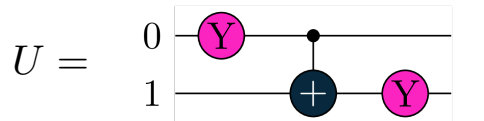
\includegraphics[width=4.16667in,height=\textheight]{circuit.png}

}

\caption{Circuit}

\end{figure}%

At this point we need to take into consideration, that Ansatz errors may
occur, since we perceive the Ansatz as an educated guess.

By computing the Eigenvalues beforehand, we were able to match the
circuit on smooth values \hspace{0pt}\hspace{0pt}at the angles 0,1,2 and
3. It should also be noted that in the following only values
\hspace{0pt}\hspace{0pt}in the interval {[}0,3{]} are considered.
Therefore, values \hspace{0pt}\hspace{0pt}outside the interval are
mapped back to the interval by applying modulo 4.

Our circuit consists of two qubits, hence we are able to have four
Eigenvalues \(\psi_{k}\). Furthermore, we know that every state has its
expectation value. Since we can regard the Hamiltonian as a Hermition
Operator we can write it as follows:\\
\[H\ket{\psi_{guess}} =  E_{guess}\ket{\psi_{guess}}\] We assume
\(E_{guess}\) to represent the expectation value of the given
Hamiltonian. Furthermore we know, that \(E_{guess}\) is a minimum under
the precondition that it approximates to a specific Eigenstate.

Our goal is to minimize the expectation value of the energy, such that
no other energy is greater than \(E_{guess}\). Therefore we will have a
solid approximation of the ground state energy. In our case the sought
Eigenvalue is the angle of the minimum Eigenstate, which corresponds to
the desired ground state energy. It can be found by applying a
minimization method to the expectation value \(E_{guess}\).

In the following graphic we can observe the plotted, expected energy
depending on the angle a. The Eigenstates are those energies
corresponding to the already calculated Eigenvalues for our circuit.

\begin{figure}[H]

{\centering 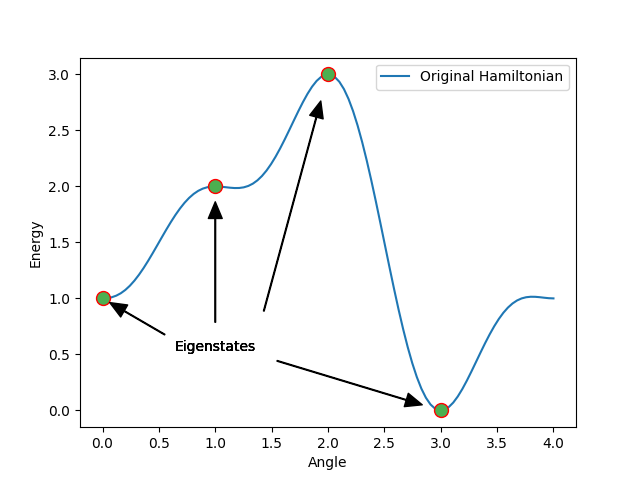
\includegraphics[width=4.16667in,height=\textheight]{Original_Hamiltonian.png}

}

\caption{Hamiltonian}

\end{figure}%

The circles in this graph represent the sought Eigenstates of \(H\).
Therefore, the corresponding angles are the targeted Eigenvalues. It is
essential to point out that the minima and maxima of this graph are
potential Eigenvalues, but they don´t neccessarily need to be. Only,
when applying different excited state methods the real Eigenvalues will
emerge. In this example we know the values. However, without prior
knowledge, we are forced to assume certain starting values. Therefore,
on one hand, it is possible to get some potential Eigenvalues at first,
which will later turn out to be irrelevant. On the other hand, saddle
points might turn into minima or maxima when applying the minimization
on multiple, consecutively executed excited state methods.

\section{Excited state methods}\label{excited-state-methods}

After having introduced the main goal and concept, we should clarify the
implementation and usage of different excited state methods. We assume,
that the Hamiltonian and our computed circuit \(U\), depending on the
angles \(\phi\), is already given in the beginning. These methods
particularly differ in the way of defining the expectation value, with
the given Hamiltonian and circuit. Also, their superposition and the
parametrization of our given circuit play a crucial role.

\subsubsection{Folded Spectrum Method}\label{folded-spectrum-method}

First we discuss the popular Folded Spectrum method. In general, it is
formulated like this: \(\langle (H-\mu)^2\rangle_{U(\phi)}\) with
\(\mu\) being the estimated value. Here it is initially assigned to 1,
since this is the first excited state in our case.\\

\begin{Shaded}
\begin{Highlighting}[]
\KeywordTok{def}\NormalTok{ expectation\_value\_folded\_spectrum(H,U, constant):}
    \ControlFlowTok{return}\NormalTok{ tq.ExpectationValue(H}\OperatorTok{=}\NormalTok{(H}\OperatorTok{{-}}\NormalTok{constant)}\OperatorTok{**}\DecValTok{2}\NormalTok{, U}\OperatorTok{=}\NormalTok{U)}
\end{Highlighting}
\end{Shaded}

\begin{figure}[H]

{\centering 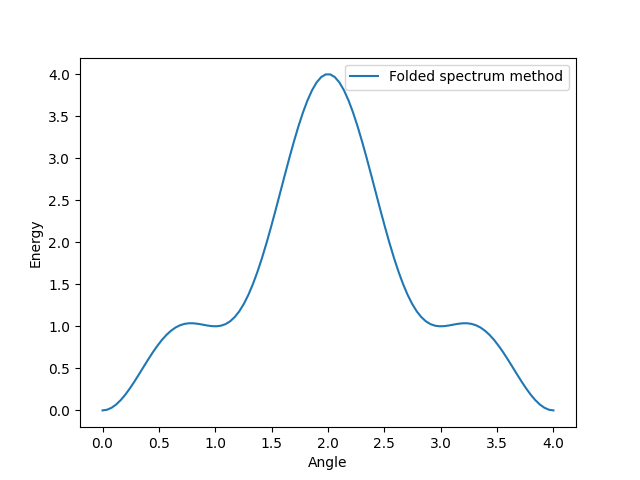
\includegraphics[width=4.16667in,height=\textheight]{Folded_spectrum.png}

}

\caption{Folded Spectrum Method}

\end{figure}%

This method modifies the Hamiltonian, by shifting its energy values. If
done properly, this concludes in the targeted excited state becoming the
lowest energy state in the plotted graph. Here, the local maximum at
angle 2.0 and local minimum at angle 3.0 are being shifted to their
initial energy value + 1.0. Simultaneously, every other value is being
shifted to the initial energy value - 1.0.

\subsubsection{Approximation Method}\label{approximation-method}

The next method is the approximation method, which differs in the way of
applying the expectation value. This looks as follows:
\((\langle H\rangle_{U(\phi)}-\mu)^2\).\\

At first we compute the expectation value of our Hamiltonian. As next
step we approximate the difference to the constant \(\mu\). This
constant is an assumption of what we think might be the target
Eigenstate. Therefore we are minimizing the difference between the
output energy of our Hamiltonian and the target energy \(\mu\).

\begin{Shaded}
\begin{Highlighting}[]
\KeywordTok{def}\NormalTok{ expectation\_value\_approximation(H,U, constant):}
    \ControlFlowTok{return}\NormalTok{ (tq.ExpectationValue(H}\OperatorTok{=}\NormalTok{H, U}\OperatorTok{=}\NormalTok{U)}\OperatorTok{{-}}\NormalTok{constant)}\OperatorTok{**}\DecValTok{2}
\end{Highlighting}
\end{Shaded}

\begin{figure}[H]

{\centering 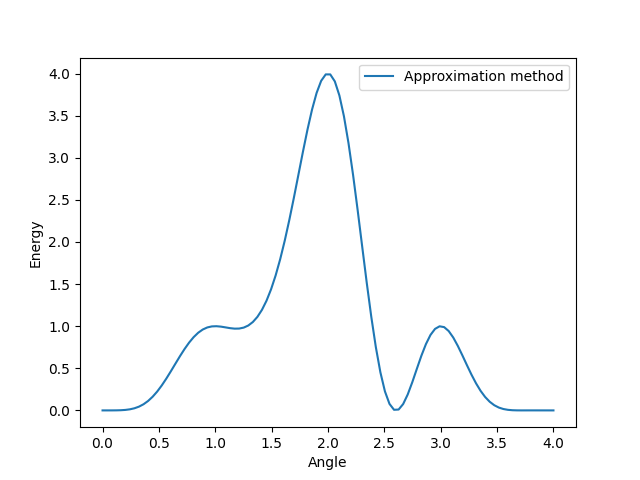
\includegraphics[width=4.16667in,height=\textheight]{Approximation.png}

}

\caption{Approximation Method}

\end{figure}%

Since we initialized \(\mu\) to 1, we mapped every energy value from 1.0
to 0.0. Thus, all affected points become the new local minima. This is
caused by minimizing the difference between our initial energy values
and the target energy \(\mu\) and \((1.0 - 1.0)^2 = 0.0\). The same
procedure is also applied to any other value of our energy graph. In the
end, the approximation affects the energy graph similarly to the Folded
Spectrum method, since it alters the initial Hamiltonian by distorting
or smoothing the spectrum. Here, the energies of the local maxima are
being shifted to their initial energy value + \(\mu\) as well. In
contrast to the Folded Spectrum method, this graph now mainly differs in
the amount of local minimas, since the Hamiltonian had two energies of
value 1.0 before.

\subsubsection{Projection Method}\label{projection-method}

Our last presented strategy is the Projection method, which is also
known as the Variational Quantum Deflation (VQD) algorithm.

This method uses a variational technique to find the k Eigenvalues of
the given Hamiltonian. With this approach we are also able to find
excited states by minimizing an objective function, which represents the
disparity between the measured expectation values and the true ground
state energy. This strategy penalizes overlapping states over several
applications of the excited state methods.\\

To find the k-th lowest excited state, VQD requires us to find the
lowest k - 1 states first. We then minimize the energy, while
constraining the state \(|\psi(\phi)\rangle\) to be orthogonal to the
lower known states \(|\psi(\phi_{i})\rangle\) :\\
\begin{align}
\underset{\phi}{\text{minimize}} & & \langle H\rangle_{\psi(\phi)} & \\
\text{subject to } & & \langle\psi(\phi_{i})~|~\psi(\phi)\rangle = 0, & \forall i \in \{ 0,\ldots k - 1\}
\end{align}\\

\strut

The constraint is given by the orthonormality of the eigenbasis of
\(H\). We can write the optimization problem as the cost function:\\

\strut

\hfill\break
\(C(\phi) = \langle\psi(\phi)|H|\psi(\phi)\rangle + \sum_{i = 0}^{k - 1}\lambda_{i}|\langle\psi(\phi_{i})|\psi(\phi)\rangle|^{2}\)\\

\strut

\hfill\break
where \(\lambda_{i}\) are the penalty weights. By optimizing over this
cost function we are able to compute the excited state energies.

\strut

\hfill\break
We define \(\left( U_{i} \right)_{i \in \{ 0,\ldots k - 1\}}\) to be the
circuits preparing the i-th state and U as the circuit preparing
\(|\psi(\phi)\rangle\).\\
The second term describes the squares of overlaps of the current circuit
U, generally known as the fidelity.\\
Referring to this \href{https://arxiv.org/pdf/2011.05938}{paper}, we get
the following conversion:

\strut

\hfill\break
\(|\braket{\psi(\phi _{i}) | \psi(\phi)}|^2\)\\
\(= \braket{\psi(\phi _{i}) | \psi(\phi)} \braket{\psi(\phi) | \psi(\phi _{i})}\)\\
\(= \bra{\psi(\phi _{i})}U_{i}\ket{0} \bra{0}U_{i}^{\textdagger}\ket{\psi(\phi _{i})}\)\\
\(=\langle P_0\rangle_{U_{i}^{\textdagger} U(\phi)}\)

The expectation values of the projected Hamiltonian can then be
described as sum of expectation values of the original Hamiltonian and
projectors of the current circuit U:\\

\(\langle H\rangle_{U(\phi)} + \sum_{i=0}^{k-1} \lambda_{i} \langle P_0\rangle_{U_{i}^{\textdagger} U(\phi)}\).

Thereby we create a sequential strategy in which the ground state is
first being calculated and then projected outwards. Therefore, a new
possible ground state is able to emerge from the projection.

\phantomsection\label{annotated-cell-5}%
\begin{Shaded}
\begin{Highlighting}[]
\KeywordTok{def}\NormalTok{ expectation\_value\_orthogonality\_constraint(H,U, circuit\_list, constant\_list):}
\NormalTok{    E }\OperatorTok{=}\NormalTok{ tq.ExpectationValue(H}\OperatorTok{=}\NormalTok{H, U}\OperatorTok{=}\NormalTok{U)}
    \ControlFlowTok{if}\NormalTok{ (}\BuiltInTok{len}\NormalTok{(circuit\_list) }\OperatorTok{!=} \BuiltInTok{len}\NormalTok{(constant\_list)):}
        \ControlFlowTok{raise} \PreprocessorTok{ValueError}\NormalTok{(}\SpecialStringTok{f"Circuit\_list and constant\_list have different lengths. len(circuit\_list): \textquotesingle{}}\SpecialCharTok{\{}\BuiltInTok{len}\NormalTok{(circuit\_list)}\SpecialCharTok{\}}\SpecialStringTok{\textquotesingle{}, len(constant\_list): \textquotesingle{}}\SpecialCharTok{\{}\BuiltInTok{len}\NormalTok{(constant\_list)}\SpecialCharTok{\}}\SpecialStringTok{\textquotesingle{}"}\NormalTok{)}
\NormalTok{    list\_length }\OperatorTok{=} \BuiltInTok{len}\NormalTok{(circuit\_list)}
    \ControlFlowTok{for}\NormalTok{ l }\KeywordTok{in} \BuiltInTok{range}\NormalTok{(list\_length):}
        \ControlFlowTok{if}\NormalTok{ (circuit\_list[l].extract\_variables() }\OperatorTok{==} \VariableTok{None}\NormalTok{):}
            \ControlFlowTok{raise} \PreprocessorTok{ValueError}\NormalTok{(}\SpecialStringTok{f"Circuit\_list contains unparametrized elements"}\NormalTok{)}
\NormalTok{    U\_list }\OperatorTok{=}\NormalTok{ []}
    \ControlFlowTok{for}\NormalTok{ i }\KeywordTok{in} \BuiltInTok{range}\NormalTok{(}\DecValTok{0}\NormalTok{, list\_length):}
\NormalTok{        U\_k }\OperatorTok{=}\NormalTok{ U }\OperatorTok{+}\NormalTok{ circuit\_list[i].dagger() }\hspace*{\fill}\NormalTok{\circled{1}}
\NormalTok{        P\_k }\OperatorTok{=} \DecValTok{1}
        \ControlFlowTok{for}\NormalTok{ k }\KeywordTok{in}\NormalTok{ U\_k.qubits:}
\NormalTok{            P\_k}\OperatorTok{*=}\NormalTok{ tq.paulis.Qp(k) }\hspace*{\fill}\NormalTok{\circled{2}}
\NormalTok{        E\_k }\OperatorTok{=}\NormalTok{ tq.ExpectationValue(H}\OperatorTok{=}\NormalTok{P\_k, U}\OperatorTok{=}\NormalTok{U\_k)}
\NormalTok{        U\_list.append(constant\_list[i]}\OperatorTok{*}\NormalTok{E\_k)}
    \ControlFlowTok{return}\NormalTok{ E }\OperatorTok{+} \BuiltInTok{sum}\NormalTok{(U\_list)}
\end{Highlighting}
\end{Shaded}

\begin{description}
\tightlist
\item[\circled{1}]
The circuit list consists of the circuits preparing the i-th state. The
addition is not an actual addition, but the concatenation operator for
quantum circuits.
\item[\circled{2}]
This is the 0-projector.
\end{description}

\begin{figure}[H]

{\centering 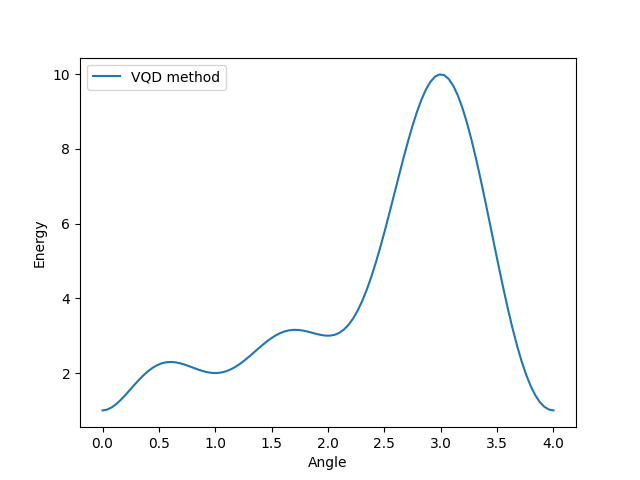
\includegraphics[width=4.16667in,height=\textheight]{VQD.png}

}

\caption{Variational Quantum Deflation Algorithm}

\end{figure}%

In our case, we already know that the energy is 0 at angle 3.0 (so we
reached a possible ground state). Hence, we set \(\lambda_{i}\) to 10,
so that the energy at angle 3.0 will become greater than any other
energy in this graph.

While the Folded Spectrum and Approximation methods are generally easier
to implement, they may have limitations in terms of accuracy and
efficiency. The Projection method offers a higher accuracy and ensures
orthogonality between the excited states, but it can be more complex and
computationally demanding, particularly for larger systems. Therefore it
is a good idea to experiment with different methods to determine the
most suitable one for a given application.

\section{Optimization process}\label{optimization-process}

Now, having discussed all possible methods, we´re going to test
different ways of concatenating those to find the ground state energy
with regard to the optimal Eigenstates and the corresponding
Eigenvalues. The whole process of finding the ground state energy
functions similarly to the popular gradient descent, since we work
stepwise through our generated graph and create a new minimum at each
iteration. For this purpose Tequila provides its own method for the
entire optimization process, the minimize-function. This method takes
the expectation value as well as a dictionary of additional parameters,
such as the initial values, as input.

\begin{Shaded}
\begin{Highlighting}[]
\KeywordTok{def}\NormalTok{ minimization(E, dict\_of\_parameters}\OperatorTok{=}\VariableTok{None}\NormalTok{):}
    \ControlFlowTok{if}\NormalTok{ dict\_of\_parameters }\KeywordTok{is} \VariableTok{None}\NormalTok{:}
\NormalTok{        dict\_of\_parameters }\OperatorTok{=}\NormalTok{ \{\}}
    \ControlFlowTok{if} \KeywordTok{not} \BuiltInTok{isinstance}\NormalTok{(dict\_of\_parameters, }\BuiltInTok{dict}\NormalTok{):}
        \ControlFlowTok{raise} \PreprocessorTok{TypeError}\NormalTok{(}\SpecialStringTok{f"dict expected, got \textquotesingle{}}\SpecialCharTok{\{}\BuiltInTok{type}\NormalTok{(dict\_of\_parameters)}\SpecialCharTok{.}\VariableTok{\_\_name\_\_}\SpecialCharTok{\}}\SpecialStringTok{\textquotesingle{}"}\NormalTok{)}
\NormalTok{    dict\_of\_parameters.setdefault(}\StringTok{"method"}\NormalTok{, }\StringTok{"BFGS"}\NormalTok{)}
\NormalTok{    dict\_of\_parameters.setdefault(}\StringTok{"initial\_values"}\NormalTok{, }\StringTok{"random"}\NormalTok{)}
    \ControlFlowTok{return}\NormalTok{ tq.minimize(E, }\OperatorTok{**}\NormalTok{dict\_of\_parameters)}
\end{Highlighting}
\end{Shaded}

Below you can first see all neccessary functions, including the excited
state methods, for the minimization as well as for plotting. Here, when
calling the main function, we pass the following input parameters:
Hamiltonian H, curcuit U, variables/angles as dictionary, a variance
threshold (optional) and list of ordered excited state methods
(optional) eg. {[}``A'',``P'',``F''{]} for Approximation, Projection,
Folded Spectrum. In this implementation, the final minimum, found after
applying the optimization on a certain excited state method, will become
the starting point of the minimization of the next method. Also, we use
the previous result energy as expectation value for the input of the
current minimization.

After the optimization process was completed successfully, you are able
to trace the derivation process of the ground state energies in the
corresponding 1D or 2D diagrams.

\begin{Shaded}
\begin{Highlighting}[]
\ImportTok{import}\NormalTok{ tequila }\ImportTok{as}\NormalTok{ tq}
\ImportTok{from}\NormalTok{ tequila }\ImportTok{import}\NormalTok{ numpy }\ImportTok{as}\NormalTok{ np}
\ImportTok{from}\NormalTok{ numpy }\ImportTok{import}\NormalTok{ pi}
\ImportTok{import}\NormalTok{ matplotlib.pyplot }\ImportTok{as}\NormalTok{ plt}
\ImportTok{import}\NormalTok{ matplotlib.pyplot }\ImportTok{as}\NormalTok{ plt}

\KeywordTok{def}\NormalTok{ main(H,U, variables, variance\_threshold}\OperatorTok{=}\FloatTok{1.e{-}8}\NormalTok{, }\BuiltInTok{list}\OperatorTok{=}\VariableTok{None}\NormalTok{):}
    \CommentTok{\textquotesingle{}\textquotesingle{}\textquotesingle{}This is the main part of this programm, where the optimization strategies "folded spectrum", "approximation" and "projection"}
\CommentTok{    are being tested and plotted.}
\CommentTok{    Input:  Hamiltonian H}
\CommentTok{            curcuit U}
\CommentTok{            variables/angles as dictionary}
\CommentTok{            variance threshold (optional)}
\CommentTok{            list of ordered functions (optional) eg. ["A","P","F"] for Approximation, Projection, Folded Spectrum}
\CommentTok{    Output: 1D or 2D graphics showing the optimization process as well as the Eigenvalues/Eigenstates of H\textquotesingle{}\textquotesingle{}\textquotesingle{}}
    
\NormalTok{    eigenvalues, vv }\OperatorTok{=}\NormalTok{ np.linalg.eigh(H.to\_matrix())}
\NormalTok{    oneDimensional }\OperatorTok{=} \VariableTok{True}
    \ControlFlowTok{if}\NormalTok{ (}\BuiltInTok{len}\NormalTok{(variables) }\OperatorTok{==} \DecValTok{2}\NormalTok{):}
\NormalTok{        oneDimensional}\OperatorTok{=}\VariableTok{False}
\NormalTok{        variables }\OperatorTok{=}\NormalTok{ \{}\StringTok{"a"}\NormalTok{: }\OperatorTok{{-}}\DecValTok{1}\NormalTok{, }\StringTok{"b"}\NormalTok{: }\OperatorTok{{-}}\FloatTok{0.5}\NormalTok{\}}
    \ControlFlowTok{else}\NormalTok{:}
\NormalTok{        variables }\OperatorTok{=}\NormalTok{ \{}\StringTok{"a"}\NormalTok{: }\OperatorTok{{-}}\DecValTok{1}\NormalTok{\}}

\NormalTok{    circuit\_list }\OperatorTok{=}\NormalTok{ []}
\NormalTok{    constant\_list }\OperatorTok{=}\NormalTok{ []}
\NormalTok{    list\_length }\OperatorTok{=} \DecValTok{4}
\NormalTok{    constant }\OperatorTok{=} \DecValTok{1}
    
    \ControlFlowTok{for}\NormalTok{ l }\KeywordTok{in} \BuiltInTok{range}\NormalTok{(list\_length):}
\NormalTok{        circuit\_list.append(U.map\_variables(variables))}
\NormalTok{        constant\_list.append(constant)}
\NormalTok{        constant }\OperatorTok{+=} \DecValTok{1}
    \ControlFlowTok{if} \BuiltInTok{list}\OperatorTok{==}\VariableTok{None}\NormalTok{:}
        \CommentTok{\# First Projection, then Approximation, then Folded Spectrum}
\NormalTok{        E }\OperatorTok{=}\NormalTok{ eigensolver.expectation\_value\_orthogonality\_constraint(H,U, circuit\_list, constant\_list)}
\NormalTok{        E\_optimized }\OperatorTok{=}\NormalTok{ eigensolver.minimization(E, \{}\StringTok{"method"}\NormalTok{:}\StringTok{"BFGS"}\NormalTok{\})}
\NormalTok{        eigensolver.plotting\_preparation(E, E\_optimized, }\StringTok{"Energy with orthogonality constraint"}\NormalTok{, eigenvalues, oneDimensional)}
        \ControlFlowTok{if}\NormalTok{ eigensolver.proof\_eigenstate(H,U, variables, variance\_threshold):}
                \BuiltInTok{print}\NormalTok{(}\StringTok{"The optimal eigenstate with a variance \textless{}= "}\NormalTok{, variance\_threshold, }\StringTok{"was found."}\NormalTok{)}
\NormalTok{        variables }\OperatorTok{=}\NormalTok{ E\_optimized.variables}
\NormalTok{        mu }\OperatorTok{=}\NormalTok{ tq.simulate(tq.ExpectationValue(H}\OperatorTok{=}\NormalTok{H, U}\OperatorTok{=}\NormalTok{U), variables}\OperatorTok{=}\NormalTok{variables)}
\NormalTok{        E\_AFS }\OperatorTok{=}\NormalTok{ eigensolver.expectation\_value\_approximation(H,U, mu)}
\NormalTok{        E\_AFS\_optimized }\OperatorTok{=}\NormalTok{ eigensolver.minimization(E\_AFS, \{}\StringTok{"method"}\NormalTok{:}\StringTok{"BFGS"}\NormalTok{, }\StringTok{"initial\_values"}\NormalTok{:variables\})}
\NormalTok{        eigensolver.plotting\_preparation(E\_AFS, E\_AFS\_optimized, }\StringTok{"Energy with approximation"}\NormalTok{, eigenvalues, oneDimensional)}
        \ControlFlowTok{if}\NormalTok{ eigensolver.proof\_eigenstate(H,U, variables, variance\_threshold):}
                \BuiltInTok{print}\NormalTok{(}\StringTok{"The optimal eigenstate with a variance \textless{}= "}\NormalTok{, variance\_threshold, }\StringTok{"was found."}\NormalTok{)}
\NormalTok{        variables }\OperatorTok{=}\NormalTok{ E\_AFS\_optimized.variables}
\NormalTok{        mu }\OperatorTok{=}\NormalTok{ tq.simulate(tq.ExpectationValue(H}\OperatorTok{=}\NormalTok{H, U}\OperatorTok{=}\NormalTok{U), variables}\OperatorTok{=}\NormalTok{variables)}
\NormalTok{        E\_FS }\OperatorTok{=}\NormalTok{ eigensolver.expectation\_value\_folded\_spectrum(H,U, mu)}
\NormalTok{        E\_FS\_optimized }\OperatorTok{=}\NormalTok{ eigensolver.minimization(E\_FS, \{}\StringTok{"method"}\NormalTok{:}\StringTok{"BFGS"}\NormalTok{, }\StringTok{"initial\_values"}\NormalTok{:variables\})}
\NormalTok{        eigensolver.plotting\_preparation(E\_FS, E\_FS\_optimized, }\StringTok{"Energy with folded spectrum"}\NormalTok{, eigenvalues, oneDimensional)}
        \ControlFlowTok{if}\NormalTok{ eigensolver.proof\_eigenstate(H,U, variables, variance\_threshold):}
                \BuiltInTok{print}\NormalTok{(}\StringTok{"The optimal eigenstate with a variance \textless{}= "}\NormalTok{, variance\_threshold, }\StringTok{"was found."}\NormalTok{)}
    \ControlFlowTok{else}\NormalTok{:}
        
        \ControlFlowTok{for}\NormalTok{ l }\KeywordTok{in} \BuiltInTok{list}\NormalTok{:}
            \ControlFlowTok{if}\NormalTok{ (l.isalpha()}\OperatorTok{==}\VariableTok{False} \KeywordTok{or} \BuiltInTok{len}\NormalTok{(l)}\OperatorTok{!=} \DecValTok{1}\NormalTok{):}
                \ControlFlowTok{raise} \PreprocessorTok{ValueError}\NormalTok{(}\StringTok{\textquotesingle{}An elemet of the list is not one letter\textquotesingle{}}\NormalTok{)}
            \ControlFlowTok{if}\NormalTok{ (l }\OperatorTok{==} \BuiltInTok{list}\NormalTok{[}\DecValTok{0}\NormalTok{]):}
\NormalTok{                mu }\OperatorTok{=} \DecValTok{1}
            \ControlFlowTok{else}\NormalTok{:}
\NormalTok{                variables }\OperatorTok{=}\NormalTok{ E\_optimized.variables}
\NormalTok{                mu }\OperatorTok{=}\NormalTok{ tq.simulate(tq.ExpectationValue(H}\OperatorTok{=}\NormalTok{H, U}\OperatorTok{=}\NormalTok{U), variables}\OperatorTok{=}\NormalTok{variables)}

            \ControlFlowTok{if}\NormalTok{ (l }\OperatorTok{==} \StringTok{"A"}\NormalTok{):}
\NormalTok{                E }\OperatorTok{=}\NormalTok{ eigensolver.expectation\_value\_approximation(H,U, mu)}
                \ControlFlowTok{if}\NormalTok{ (l }\OperatorTok{==} \BuiltInTok{list}\NormalTok{[}\DecValTok{0}\NormalTok{]):}
\NormalTok{                    E\_optimized }\OperatorTok{=}\NormalTok{ eigensolver.minimization(E, \{}\StringTok{"method"}\NormalTok{:}\StringTok{"BFGS"}\NormalTok{\})}
                \ControlFlowTok{else}\NormalTok{: }
\NormalTok{                    E\_optimized }\OperatorTok{=}\NormalTok{ eigensolver.minimization(E, \{}\StringTok{"method"}\NormalTok{:}\StringTok{"BFGS"}\NormalTok{, }\StringTok{"initial\_values"}\NormalTok{:variables\})}
\NormalTok{                eigensolver.plotting\_preparation(E, E\_optimized, }\StringTok{"Energy with approximation"}\NormalTok{, eigenvalues, oneDimensional)}
                \ControlFlowTok{if}\NormalTok{ eigensolver.proof\_eigenstate(H,U, variables, variance\_threshold):}
                        \BuiltInTok{print}\NormalTok{(}\StringTok{"The optimal eigenstate with a variance \textless{}= "}\NormalTok{, variance\_threshold, }\StringTok{"was found."}\NormalTok{)}
            \ControlFlowTok{elif}\NormalTok{ (l }\OperatorTok{==} \StringTok{"P"}\NormalTok{):}
\NormalTok{                E }\OperatorTok{=}\NormalTok{ eigensolver.expectation\_value\_orthogonality\_constraint(H,U, circuit\_list, constant\_list)}
                \ControlFlowTok{if}\NormalTok{ (l }\OperatorTok{==} \BuiltInTok{list}\NormalTok{[}\DecValTok{0}\NormalTok{]):}
\NormalTok{                    E\_optimized }\OperatorTok{=}\NormalTok{ eigensolver.minimization(E, \{}\StringTok{"method"}\NormalTok{:}\StringTok{"BFGS"}\NormalTok{\})}
                \ControlFlowTok{else}\NormalTok{: }
\NormalTok{                    E\_optimized }\OperatorTok{=}\NormalTok{ eigensolver.minimization(E, \{}\StringTok{"method"}\NormalTok{:}\StringTok{"BFGS"}\NormalTok{, }\StringTok{"initial\_values"}\NormalTok{:variables\})}
\NormalTok{                eigensolver.plotting\_preparation(E, E\_optimized, }\StringTok{"Energy with orthogonality constraint"}\NormalTok{, eigenvalues, oneDimensional)}
                \ControlFlowTok{if}\NormalTok{ eigensolver.proof\_eigenstate(H,U, variables, variance\_threshold):}
                        \BuiltInTok{print}\NormalTok{(}\StringTok{"The optimal eigenstate with a variance \textless{}= "}\NormalTok{, variance\_threshold, }\StringTok{"was found."}\NormalTok{)}
            \ControlFlowTok{elif}\NormalTok{ (l }\OperatorTok{==} \StringTok{"F"}\NormalTok{):}
\NormalTok{                E }\OperatorTok{=}\NormalTok{ eigensolver.expectation\_value\_folded\_spectrum(H,U, mu)}
                \ControlFlowTok{if}\NormalTok{ (l }\OperatorTok{==} \BuiltInTok{list}\NormalTok{[}\DecValTok{0}\NormalTok{]):}
\NormalTok{                    E\_optimized }\OperatorTok{=}\NormalTok{ eigensolver.minimization(E, \{}\StringTok{"method"}\NormalTok{:}\StringTok{"BFGS"}\NormalTok{\})}
                \ControlFlowTok{else}\NormalTok{: }
\NormalTok{                    E\_optimized }\OperatorTok{=}\NormalTok{ eigensolver.minimization(E, \{}\StringTok{"method"}\NormalTok{:}\StringTok{"BFGS"}\NormalTok{, }\StringTok{"initial\_values"}\NormalTok{:variables\})}
\NormalTok{                eigensolver.plotting\_preparation(E, E\_optimized, }\StringTok{"Energy with folded spectrum"}\NormalTok{, eigenvalues, oneDimensional)}
                \ControlFlowTok{if}\NormalTok{ eigensolver.proof\_eigenstate(H,U, variables, variance\_threshold):}
                        \BuiltInTok{print}\NormalTok{(}\StringTok{"The optimal eigenstate with a variance \textless{}= "}\NormalTok{, variance\_threshold, }\StringTok{"was found."}\NormalTok{)}
                
            \ControlFlowTok{else}\NormalTok{:}
                \ControlFlowTok{raise} \PreprocessorTok{ValueError}\NormalTok{(}\StringTok{\textquotesingle{}An elemet of the list is not letter "A", "P" or "F"\textquotesingle{}}\NormalTok{)}

\CommentTok{\#{-}{-}{-}{-}{-}{-}{-}{-}{-}{-}{-}{-}{-}{-}{-}{-}General functions{-}{-}{-}{-}{-}{-}{-}{-}{-}{-}{-}{-}}
\KeywordTok{class}\NormalTok{ eigensolver:}
    
    \KeywordTok{def}\NormalTok{ expectation\_value\_folded\_spectrum(H,U, constant):}
        \ControlFlowTok{return}\NormalTok{ tq.ExpectationValue(H}\OperatorTok{=}\NormalTok{(H}\OperatorTok{{-}}\NormalTok{constant)}\OperatorTok{**}\DecValTok{2}\NormalTok{, U}\OperatorTok{=}\NormalTok{U)}
    
    \KeywordTok{def}\NormalTok{ expectation\_value\_approximation(H,U, constant):}
        \ControlFlowTok{return}\NormalTok{ (tq.ExpectationValue(H}\OperatorTok{=}\NormalTok{H, U}\OperatorTok{=}\NormalTok{U)}\OperatorTok{{-}}\NormalTok{constant)}\OperatorTok{**}\DecValTok{2}
    
    \KeywordTok{def}\NormalTok{ expectation\_value\_orthogonality\_constraint(H,U, circuit\_list, constant\_list):}
\NormalTok{        E }\OperatorTok{=}\NormalTok{ tq.ExpectationValue(H}\OperatorTok{=}\NormalTok{H, U}\OperatorTok{=}\NormalTok{U)}
        \ControlFlowTok{if}\NormalTok{ (}\BuiltInTok{len}\NormalTok{(circuit\_list) }\OperatorTok{!=} \BuiltInTok{len}\NormalTok{(constant\_list)):}
            \ControlFlowTok{raise} \PreprocessorTok{ValueError}\NormalTok{(}\SpecialStringTok{f"Circuit\_list and constant\_list have different lengths. len(circuit\_list): \textquotesingle{}}\SpecialCharTok{\{}\BuiltInTok{len}\NormalTok{(circuit\_list)}\SpecialCharTok{\}}\SpecialStringTok{\textquotesingle{}, len(constant\_list): \textquotesingle{}}\SpecialCharTok{\{}\BuiltInTok{len}\NormalTok{(constant\_list)}\SpecialCharTok{\}}\SpecialStringTok{\textquotesingle{}"}\NormalTok{)}
\NormalTok{        list\_length }\OperatorTok{=} \BuiltInTok{len}\NormalTok{(circuit\_list)}
        \ControlFlowTok{for}\NormalTok{ l }\KeywordTok{in} \BuiltInTok{range}\NormalTok{(list\_length):}
            \ControlFlowTok{if}\NormalTok{ (circuit\_list[l].extract\_variables() }\OperatorTok{==} \VariableTok{None}\NormalTok{):}
                \ControlFlowTok{raise} \PreprocessorTok{ValueError}\NormalTok{(}\SpecialStringTok{f"Circuit\_list contains unparametrized elements"}\NormalTok{)}
\NormalTok{        U\_list }\OperatorTok{=}\NormalTok{ []}
        \ControlFlowTok{for}\NormalTok{ i }\KeywordTok{in} \BuiltInTok{range}\NormalTok{(}\DecValTok{0}\NormalTok{, list\_length):}
\NormalTok{            U\_k }\OperatorTok{=}\NormalTok{ U }\OperatorTok{+}\NormalTok{ circuit\_list[i].dagger()}
\NormalTok{            P\_k }\OperatorTok{=} \DecValTok{1}
            \ControlFlowTok{for}\NormalTok{ k }\KeywordTok{in}\NormalTok{ U\_k.qubits:}
\NormalTok{                P\_k}\OperatorTok{*=}\NormalTok{ tq.paulis.Qp(k)}
\NormalTok{            E\_k }\OperatorTok{=}\NormalTok{ tq.ExpectationValue(H}\OperatorTok{=}\NormalTok{P\_k, U}\OperatorTok{=}\NormalTok{U\_k)}
\NormalTok{            U\_list.append(constant\_list[i]}\OperatorTok{*}\NormalTok{E\_k)}
        \ControlFlowTok{return}\NormalTok{ E }\OperatorTok{+} \BuiltInTok{sum}\NormalTok{(U\_list)}

    \KeywordTok{def}\NormalTok{ minimization(E, dict\_of\_parameters}\OperatorTok{=}\VariableTok{None}\NormalTok{):}
        \ControlFlowTok{if}\NormalTok{ dict\_of\_parameters }\KeywordTok{is} \VariableTok{None}\NormalTok{:}
\NormalTok{            dict\_of\_parameters }\OperatorTok{=}\NormalTok{ \{\}}
        \ControlFlowTok{if} \KeywordTok{not} \BuiltInTok{isinstance}\NormalTok{(dict\_of\_parameters, }\BuiltInTok{dict}\NormalTok{):}
            \ControlFlowTok{raise} \PreprocessorTok{TypeError}\NormalTok{(}\SpecialStringTok{f"dict expected, got \textquotesingle{}}\SpecialCharTok{\{}\BuiltInTok{type}\NormalTok{(dict\_of\_parameters)}\SpecialCharTok{.}\VariableTok{\_\_name\_\_}\SpecialCharTok{\}}\SpecialStringTok{\textquotesingle{}"}\NormalTok{)}
\NormalTok{        dict\_of\_parameters.setdefault(}\StringTok{"method"}\NormalTok{, }\StringTok{"BFGS"}\NormalTok{)}
\NormalTok{        dict\_of\_parameters.setdefault(}\StringTok{"initial\_values"}\NormalTok{, }\StringTok{"random"}\NormalTok{)}
        \ControlFlowTok{return}\NormalTok{ tq.minimize(E, }\OperatorTok{**}\NormalTok{dict\_of\_parameters)}
    
    
    \KeywordTok{def}\NormalTok{ proof\_eigenstate(H, U, variables, variance\_threshold}\OperatorTok{=}\FloatTok{1.e{-}4}\NormalTok{):}
\NormalTok{        V }\OperatorTok{=}\NormalTok{ ((tq.ExpectationValue(H}\OperatorTok{=}\NormalTok{H, U}\OperatorTok{=}\NormalTok{U))  }\OperatorTok{**}\DecValTok{2} \OperatorTok{{-}}\NormalTok{ tq.ExpectationValue(H}\OperatorTok{=}\NormalTok{H}\OperatorTok{**}\DecValTok{2}\NormalTok{, U}\OperatorTok{=}\NormalTok{U)).}\BuiltInTok{apply}\NormalTok{(}\BuiltInTok{abs}\NormalTok{)}
\NormalTok{        V }\OperatorTok{=}\NormalTok{ tq.simulate(V, variables)}
        \ControlFlowTok{return}\NormalTok{ V }\OperatorTok{\textless{}=}\NormalTok{ variance\_threshold}
    
    \KeywordTok{def}\NormalTok{ get\_optimization\_energies(result):}
        \ControlFlowTok{return}\NormalTok{ result.history.energies\_calls}

    \KeywordTok{def}\NormalTok{ get\_optimization\_angles(result, eigenvalues):}
\NormalTok{        mod }\OperatorTok{=} \BuiltInTok{len}\NormalTok{(eigenvalues)}
\NormalTok{        angle\_dots }\OperatorTok{=}\NormalTok{ [\{k:v }\OperatorTok{\%}\NormalTok{ mod }\ControlFlowTok{for}\NormalTok{ k,v }\KeywordTok{in}\NormalTok{ x.items()\} }\ControlFlowTok{for}\NormalTok{ x }\KeywordTok{in}\NormalTok{ result.history.angles\_calls]}
\NormalTok{        angles\_np }\OperatorTok{=}\NormalTok{ np.array([}\BuiltInTok{list}\NormalTok{(i.values()) }\ControlFlowTok{for}\NormalTok{ i }\KeywordTok{in}\NormalTok{ angle\_dots])}
        \ControlFlowTok{return}\NormalTok{ angles\_np}
    
    \KeywordTok{def}\NormalTok{ compile\_E\_values1D(fE, angle\_range):}
        \ControlFlowTok{return}\NormalTok{ [fE(\{}\StringTok{"a"}\NormalTok{:v\}) }\ControlFlowTok{for}\NormalTok{ v }\KeywordTok{in}\NormalTok{ angle\_range]}
    
    \KeywordTok{def}\NormalTok{ compile\_E\_values2D(fE, angle\_range):}
\NormalTok{        fE\_result }\OperatorTok{=}\NormalTok{ []}
        \ControlFlowTok{for}\NormalTok{ v }\KeywordTok{in}\NormalTok{ angle\_range:}
            \ControlFlowTok{for}\NormalTok{ w }\KeywordTok{in}\NormalTok{ angle\_range:}
\NormalTok{                fE\_result.append(fE(\{}\StringTok{"a"}\NormalTok{:v, }\StringTok{"b"}\NormalTok{:w\}))}
                \ControlFlowTok{return}\NormalTok{ fE\_result}

    \KeywordTok{def}\NormalTok{ compile\_dE\_values1D(fdE, angle\_range):}
        \ControlFlowTok{return}\NormalTok{ [fdE(\{}\StringTok{"a"}\NormalTok{:v\}) }\ControlFlowTok{for}\NormalTok{ v }\KeywordTok{in}\NormalTok{ angle\_range]}
    
    \KeywordTok{def}\NormalTok{ compile\_dE\_values2D(fdE, angle\_range):}
\NormalTok{        fE\_result }\OperatorTok{=}\NormalTok{ []}
        \ControlFlowTok{for}\NormalTok{ v }\KeywordTok{in}\NormalTok{ angle\_range:}
            \ControlFlowTok{for}\NormalTok{ w }\KeywordTok{in}\NormalTok{ angle\_range:}
\NormalTok{                fE\_result.append(fdE(\{}\StringTok{"a"}\NormalTok{:v, }\StringTok{"b"}\NormalTok{:w\}))}
                \ControlFlowTok{return}\NormalTok{ fE\_result}
    
    \CommentTok{\# calculating min and max values of range of all energies (E or dE) for plotting. Returning array [y\_min, y\_max]}
    \KeywordTok{def}\NormalTok{ min\_max\_y\_value(E, values\_E, values\_dE, energy\_dots):}
\NormalTok{        min\_max }\OperatorTok{=}\NormalTok{ []}
\NormalTok{        all\_energy\_values }\OperatorTok{=}\NormalTok{ []}
        \ControlFlowTok{for}\NormalTok{ v }\KeywordTok{in}\NormalTok{ values\_E:}
\NormalTok{            all\_energy\_values.append(v)}
        \ControlFlowTok{for}\NormalTok{ v }\KeywordTok{in}\NormalTok{ values\_dE:}
\NormalTok{            all\_energy\_values.append(v)}
\NormalTok{        y\_min }\OperatorTok{=}\NormalTok{ energy\_dots[}\DecValTok{0}\NormalTok{]}
\NormalTok{        y\_max }\OperatorTok{=}\NormalTok{ energy\_dots[}\DecValTok{0}\NormalTok{]}
        \ControlFlowTok{for}\NormalTok{ energy }\KeywordTok{in}\NormalTok{ all\_energy\_values:}
            \ControlFlowTok{if}\NormalTok{ energy }\OperatorTok{\textless{}}\NormalTok{ y\_min:}
\NormalTok{                y\_min }\OperatorTok{=}\NormalTok{ energy}
            \ControlFlowTok{if}\NormalTok{ energy }\OperatorTok{\textgreater{}}\NormalTok{ y\_max:}
\NormalTok{                y\_max }\OperatorTok{=}\NormalTok{ energy}
\NormalTok{        min\_max.append(y\_min)}
\NormalTok{        min\_max.append(y\_max)}
        \ControlFlowTok{return}\NormalTok{ min\_max}
    
    \KeywordTok{def}\NormalTok{ plotting1D(aprox\_name, angle\_range, angles\_np, values\_E, values\_dE, fE, energy\_np, start\_dot\_E, end\_dot\_E, start\_dot\_angle, end\_dot\_angle, angles\_of\_eigenvalues, y\_min, y\_max):}
        
\NormalTok{        plt.plot(angle\_range, values\_E, label}\OperatorTok{=} \BuiltInTok{str}\NormalTok{(aprox\_name))}
        
\NormalTok{        plt.plot(angle\_range, values\_dE, label}\OperatorTok{=} \StringTok{\textquotesingle{}Derivation of the \textquotesingle{}} \OperatorTok{+} \BuiltInTok{str}\NormalTok{(aprox\_name))}
\NormalTok{        plt.legend([}\BuiltInTok{str}\NormalTok{(aprox\_name), }\StringTok{\textquotesingle{}Derivation of the \textquotesingle{}} \OperatorTok{+} \BuiltInTok{str}\NormalTok{(aprox\_name)])}
\NormalTok{        plt.scatter(angles\_np, energy\_np)}
        
        \ControlFlowTok{for}\NormalTok{ a }\KeywordTok{in}\NormalTok{ angles\_of\_eigenvalues:}
\NormalTok{            plt.plot(a, fE(\{}\StringTok{"a"}\NormalTok{:a\}), }\StringTok{"o"}\NormalTok{,mfc }\OperatorTok{=} \StringTok{\textquotesingle{}\#4CAF50\textquotesingle{}}\NormalTok{,ms }\OperatorTok{=} \DecValTok{10}\NormalTok{,mec }\OperatorTok{=} \StringTok{\textquotesingle{}r\textquotesingle{}}\NormalTok{)}
\NormalTok{            plt.vlines(x}\OperatorTok{=}\NormalTok{a, colors}\OperatorTok{=}\StringTok{\textquotesingle{}purple\textquotesingle{}}\NormalTok{, ymin}\OperatorTok{=}\NormalTok{y\_min}\OperatorTok{{-}}\DecValTok{5}\NormalTok{, ymax}\OperatorTok{=}\NormalTok{y\_max}\OperatorTok{+}\DecValTok{5}\NormalTok{, ls}\OperatorTok{=}\StringTok{\textquotesingle{}{-}{-}\textquotesingle{}}\NormalTok{, lw}\OperatorTok{=}\DecValTok{2}\NormalTok{, label}\OperatorTok{=}\StringTok{\textquotesingle{}Eigenvalues\textquotesingle{}}\NormalTok{)}
\NormalTok{        plt.annotate(}\StringTok{\textquotesingle{}Starting point\textquotesingle{}}\NormalTok{,}
\NormalTok{        ha }\OperatorTok{=} \StringTok{\textquotesingle{}center\textquotesingle{}}\NormalTok{, va }\OperatorTok{=} \StringTok{\textquotesingle{}bottom\textquotesingle{}}\NormalTok{,}
\NormalTok{        xytext }\OperatorTok{=}\NormalTok{ (start\_dot\_angle , start\_dot\_E }\OperatorTok{{-}} \DecValTok{2}\NormalTok{),}
\NormalTok{        xy }\OperatorTok{=}\NormalTok{ (start\_dot\_angle, start\_dot\_E),}
\NormalTok{        arrowprops }\OperatorTok{=}\NormalTok{ \{ }\StringTok{\textquotesingle{}facecolor\textquotesingle{}}\NormalTok{ : }\StringTok{\textquotesingle{}black\textquotesingle{}}\NormalTok{, }\StringTok{\textquotesingle{}shrink\textquotesingle{}}\NormalTok{ : }\FloatTok{0.5}\NormalTok{, }\StringTok{\textquotesingle{}width\textquotesingle{}}\NormalTok{ : }\FloatTok{0.5}\NormalTok{, }\StringTok{\textquotesingle{}headwidth\textquotesingle{}}\NormalTok{ : }\DecValTok{10}\NormalTok{\})}
\NormalTok{        plt.annotate(}\StringTok{\textquotesingle{}End point\textquotesingle{}}\NormalTok{,}
\NormalTok{        ha }\OperatorTok{=} \StringTok{\textquotesingle{}center\textquotesingle{}}\NormalTok{, va }\OperatorTok{=} \StringTok{\textquotesingle{}bottom\textquotesingle{}}\NormalTok{,}
\NormalTok{        xytext }\OperatorTok{=}\NormalTok{ (end\_dot\_angle, end\_dot\_E }\OperatorTok{+} \DecValTok{2}\NormalTok{),}
\NormalTok{        xy }\OperatorTok{=}\NormalTok{ (end\_dot\_angle, end\_dot\_E),}
\NormalTok{        arrowprops }\OperatorTok{=}\NormalTok{ \{ }\StringTok{\textquotesingle{}facecolor\textquotesingle{}}\NormalTok{ : }\StringTok{\textquotesingle{}black\textquotesingle{}}\NormalTok{, }\StringTok{\textquotesingle{}shrink\textquotesingle{}}\NormalTok{ : }\FloatTok{0.5}\NormalTok{, }\StringTok{\textquotesingle{}width\textquotesingle{}}\NormalTok{ : }\FloatTok{0.5}\NormalTok{, }\StringTok{\textquotesingle{}headwidth\textquotesingle{}}\NormalTok{ : }\DecValTok{10}\NormalTok{\})}
        
\NormalTok{        plt.xlabel(}\StringTok{"Eigenvalues"}\NormalTok{)}
\NormalTok{        plt.ylabel(}\StringTok{"Eigenstates"}\NormalTok{)}
\NormalTok{        plt.show()}

    \KeywordTok{def}\NormalTok{ plotting1Dnew(aprox\_name, angle\_range, values\_E):}
        
\NormalTok{        plt.plot(angle\_range, values\_E, label}\OperatorTok{=} \BuiltInTok{str}\NormalTok{(aprox\_name))}
\NormalTok{        plt.legend([}\BuiltInTok{str}\NormalTok{(aprox\_name)])}
        
\NormalTok{        plt.xlabel(}\StringTok{"Angle"}\NormalTok{)}
\NormalTok{        plt.ylabel(}\StringTok{"Energy"}\NormalTok{)}
\NormalTok{        plt.show()}

    \KeywordTok{def}\NormalTok{ plotting2D(aprox\_name, start\_dot\_E, end\_dot\_E, start\_dot\_angle, end\_dot\_angle, fE, angles\_of\_eigenvalues):}
\NormalTok{        X}\OperatorTok{=}\NormalTok{np.linspace(}\FloatTok{0.0}\NormalTok{, }\FloatTok{2.0}\OperatorTok{*}\NormalTok{np.pi,}\DecValTok{25}\NormalTok{)}
\NormalTok{        Y}\OperatorTok{=}\NormalTok{X}
\NormalTok{        Z }\OperatorTok{=}\NormalTok{ np.zeros([}\DecValTok{25}\NormalTok{,}\DecValTok{25}\NormalTok{])}
        \ControlFlowTok{for}\NormalTok{ i,x }\KeywordTok{in} \BuiltInTok{enumerate}\NormalTok{(X):}
            \ControlFlowTok{for}\NormalTok{ j,y }\KeywordTok{in} \BuiltInTok{enumerate}\NormalTok{(Y):}
\NormalTok{                Z[i,j]}\OperatorTok{=}\NormalTok{ fE(\{}\StringTok{"a"}\NormalTok{:x, }\StringTok{"b"}\NormalTok{:y\})}
\NormalTok{        X, Y }\OperatorTok{=}\NormalTok{ np.meshgrid(X, Y)}
\NormalTok{        ax }\OperatorTok{=}\NormalTok{ plt.figure().add\_subplot(projection}\OperatorTok{=}\StringTok{\textquotesingle{}3d\textquotesingle{}}\NormalTok{)}
\NormalTok{        ax.plot\_surface(X, Y, Z, edgecolor}\OperatorTok{=}\StringTok{\textquotesingle{}royalblue\textquotesingle{}}\NormalTok{, lw}\OperatorTok{=}\FloatTok{0.5}\NormalTok{, rstride}\OperatorTok{=}\DecValTok{8}\NormalTok{, cstride}\OperatorTok{=}\DecValTok{8}\NormalTok{,}
\NormalTok{                        alpha}\OperatorTok{=}\FloatTok{0.3}\NormalTok{, shade}\OperatorTok{=}\VariableTok{True}\NormalTok{)}
        
        \ControlFlowTok{for}\NormalTok{ a }\KeywordTok{in}\NormalTok{ angles\_of\_eigenvalues:}
            \ControlFlowTok{for}\NormalTok{ b }\KeywordTok{in}\NormalTok{ angles\_of\_eigenvalues:}
                \ControlFlowTok{if}\NormalTok{ (a }\OperatorTok{==}\NormalTok{ angles\_of\_eigenvalues[}\DecValTok{0}\NormalTok{] }\KeywordTok{and}\NormalTok{ b }\OperatorTok{==}\NormalTok{ angles\_of\_eigenvalues[}\DecValTok{0}\NormalTok{]):}
\NormalTok{                    ax.plot(a,b, fE(\{}\StringTok{"a"}\NormalTok{:a, }\StringTok{"b"}\NormalTok{:b\}), }\StringTok{"o"}\NormalTok{,mfc }\OperatorTok{=} \StringTok{\textquotesingle{}\#4CAF50\textquotesingle{}}\NormalTok{,ms }\OperatorTok{=} \DecValTok{10}\NormalTok{,mec }\OperatorTok{=} \StringTok{\textquotesingle{}r\textquotesingle{}}\NormalTok{,label}\OperatorTok{=}\StringTok{"Possible Eigenvalues"}\NormalTok{)}
                \ControlFlowTok{else}\NormalTok{:}
\NormalTok{                    ax.plot(a,b, fE(\{}\StringTok{"a"}\NormalTok{:a, }\StringTok{"b"}\NormalTok{:b\}), }\StringTok{"o"}\NormalTok{,mfc }\OperatorTok{=} \StringTok{\textquotesingle{}\#4CAF50\textquotesingle{}}\NormalTok{,ms }\OperatorTok{=} \DecValTok{10}\NormalTok{,mec }\OperatorTok{=} \StringTok{\textquotesingle{}r\textquotesingle{}}\NormalTok{)}

        \ControlFlowTok{if}\NormalTok{ (fE(\{}\StringTok{"a"}\NormalTok{:end\_dot\_angle[}\DecValTok{0}\NormalTok{], }\StringTok{"b"}\NormalTok{:end\_dot\_angle[}\DecValTok{1}\NormalTok{]\}) }\OperatorTok{==}\NormalTok{ fE(\{}\StringTok{"a"}\NormalTok{:start\_dot\_angle[}\DecValTok{0}\NormalTok{], }\StringTok{"b"}\NormalTok{:start\_dot\_angle[}\DecValTok{1}\NormalTok{]\})):}
\NormalTok{            ax.scatter3D(start\_dot\_angle[}\DecValTok{0}\NormalTok{], start\_dot\_angle[}\DecValTok{1}\NormalTok{],fE(\{}\StringTok{"a"}\NormalTok{:start\_dot\_angle[}\DecValTok{0}\NormalTok{], }\StringTok{"b"}\NormalTok{:start\_dot\_angle[}\DecValTok{1}\NormalTok{]\}),color}\OperatorTok{=}\StringTok{\textquotesingle{}red\textquotesingle{}}\NormalTok{, s}\OperatorTok{=}\DecValTok{25}\NormalTok{, label}\OperatorTok{=}\StringTok{"Starting point equals End point"}\NormalTok{)}
        \ControlFlowTok{else}\NormalTok{:}
\NormalTok{            ax.scatter3D(end\_dot\_angle[}\DecValTok{0}\NormalTok{], end\_dot\_angle[}\DecValTok{1}\NormalTok{],fE(\{}\StringTok{"a"}\NormalTok{:end\_dot\_angle[}\DecValTok{0}\NormalTok{], }\StringTok{"b"}\NormalTok{:end\_dot\_angle[}\DecValTok{1}\NormalTok{]\}),color}\OperatorTok{=}\StringTok{\textquotesingle{}black\textquotesingle{}}\NormalTok{, s}\OperatorTok{=}\DecValTok{25}\NormalTok{, label}\OperatorTok{=}\StringTok{"Starting point"}\NormalTok{)}
\NormalTok{            ax.scatter3D(start\_dot\_angle[}\DecValTok{0}\NormalTok{], start\_dot\_angle[}\DecValTok{1}\NormalTok{],fE(\{}\StringTok{"a"}\NormalTok{:start\_dot\_angle[}\DecValTok{0}\NormalTok{], }\StringTok{"b"}\NormalTok{:start\_dot\_angle[}\DecValTok{1}\NormalTok{]\}),color}\OperatorTok{=}\StringTok{\textquotesingle{}red\textquotesingle{}}\NormalTok{, s}\OperatorTok{=}\DecValTok{25}\NormalTok{, label}\OperatorTok{=}\StringTok{"End point"}\NormalTok{)}


\NormalTok{        ax.set\_xlabel(}\StringTok{\textquotesingle{}Angle "a"\textquotesingle{}}\NormalTok{)}
\NormalTok{        ax.set\_ylabel(}\StringTok{\textquotesingle{}Angle "b"\textquotesingle{}}\NormalTok{)}
\NormalTok{        ax.set\_zlabel(}\StringTok{\textquotesingle{}Energy\textquotesingle{}}\NormalTok{)}
\NormalTok{        ax.legend()}
\NormalTok{        plt.show()}

    \KeywordTok{def}\NormalTok{ plotting\_preparation(E, result, aprox\_name, eigenvalues, oneDimensional}\OperatorTok{=}\VariableTok{True}\NormalTok{):}
\NormalTok{        angle\_range }\OperatorTok{=}\NormalTok{ (np.linspace(}\DecValTok{0}\NormalTok{,}\DecValTok{4}\NormalTok{,}\DecValTok{100}\NormalTok{))}
\NormalTok{        angles\_of\_eigenvalues }\OperatorTok{=}\NormalTok{ eigenvalues}

\NormalTok{        fE }\OperatorTok{=}\NormalTok{ tq.}\BuiltInTok{compile}\NormalTok{(E)}
        
        \ControlFlowTok{if}\NormalTok{ oneDimensional:}
\NormalTok{            values\_E }\OperatorTok{=}\NormalTok{ eigensolver.compile\_E\_values1D(fE, angle\_range)}
\NormalTok{            dE }\OperatorTok{=}\NormalTok{ tq.grad(E, }\StringTok{"a"}\NormalTok{)}
        \ControlFlowTok{else}\NormalTok{:}
\NormalTok{            values\_E }\OperatorTok{=}\NormalTok{ eigensolver.compile\_E\_values2D(fE, angle\_range)}
\NormalTok{            dE }\OperatorTok{=}\NormalTok{ tq.grad(E, }\StringTok{"a"}\NormalTok{, }\StringTok{"b"}\NormalTok{)}
\NormalTok{        fdE }\OperatorTok{=}\NormalTok{ tq.}\BuiltInTok{compile}\NormalTok{(dE)}
        \ControlFlowTok{if}\NormalTok{ oneDimensional:}
\NormalTok{            values\_dE }\OperatorTok{=}\NormalTok{ eigensolver.compile\_dE\_values1D(fdE, angle\_range)}
        \ControlFlowTok{else}\NormalTok{:}
\NormalTok{            values\_dE }\OperatorTok{=}\NormalTok{ eigensolver.compile\_dE\_values2D(fdE, angle\_range)}
        
\NormalTok{        angles }\OperatorTok{=}\NormalTok{ eigensolver.get\_optimization\_angles(result, eigenvalues)}
\NormalTok{        energy\_dots }\OperatorTok{=}\NormalTok{ eigensolver.get\_optimization\_energies(result)}
        
        \ControlFlowTok{if}\NormalTok{ oneDimensional:}
\NormalTok{            angles\_np }\OperatorTok{=}\NormalTok{ []}
            \ControlFlowTok{for}\NormalTok{ xs }\KeywordTok{in}\NormalTok{ angles:}
                \ControlFlowTok{for}\NormalTok{ x }\KeywordTok{in}\NormalTok{ xs:}
\NormalTok{                    angles\_np.append(x)}
        \ControlFlowTok{else}\NormalTok{:}
\NormalTok{            angles\_np }\OperatorTok{=}\NormalTok{ angles}

\NormalTok{        y\_min }\OperatorTok{=}\NormalTok{ eigensolver.min\_max\_y\_value(E, values\_E, values\_dE, energy\_dots)[}\DecValTok{0}\NormalTok{]}
\NormalTok{        y\_max }\OperatorTok{=}\NormalTok{ eigensolver.min\_max\_y\_value(E, values\_E, values\_dE, energy\_dots)[}\DecValTok{1}\NormalTok{]}
        
\NormalTok{        start\_dot\_E }\OperatorTok{=}\NormalTok{ energy\_dots[}\DecValTok{0}\NormalTok{]}
\NormalTok{        end\_dot\_E }\OperatorTok{=}\NormalTok{ energy\_dots[}\BuiltInTok{len}\NormalTok{(energy\_dots)}\OperatorTok{{-}}\DecValTok{1}\NormalTok{]}
\NormalTok{        start\_dot\_angle }\OperatorTok{=}\NormalTok{ angles\_np[}\DecValTok{0}\NormalTok{]}
\NormalTok{        end\_dot\_angle }\OperatorTok{=}\NormalTok{ angles\_np[}\BuiltInTok{len}\NormalTok{(energy\_dots)}\OperatorTok{{-}}\DecValTok{1}\NormalTok{]}
        
        \ControlFlowTok{if}\NormalTok{ oneDimensional:}
\NormalTok{            eigensolver.plotting1D(aprox\_name, angle\_range, angles\_np, values\_E, values\_dE, fE, energy\_dots, start\_dot\_E, end\_dot\_E, start\_dot\_angle, end\_dot\_angle, angles\_of\_eigenvalues, y\_min, y\_max)}
        \ControlFlowTok{else}\NormalTok{:}
\NormalTok{            eigensolver.plotting2D(aprox\_name, start\_dot\_E, end\_dot\_E, start\_dot\_angle, end\_dot\_angle, fE, angles\_of\_eigenvalues)}
    

    \KeywordTok{def}\NormalTok{ min\_max\_energy\_and\_angle(fE,values\_E, angle\_range):}
\NormalTok{        min\_E }\OperatorTok{=} \BuiltInTok{min}\NormalTok{(np.array(values\_E))}

        \ControlFlowTok{for}\NormalTok{ a }\KeywordTok{in}\NormalTok{ angle\_range:}
            \ControlFlowTok{if}\NormalTok{ (fE(\{}\StringTok{"a"}\NormalTok{:a\}) }\OperatorTok{==}\NormalTok{ min\_E):}
\NormalTok{                min\_angle }\OperatorTok{=}\NormalTok{ a}
                \ControlFlowTok{break}
\NormalTok{        max\_E }\OperatorTok{=} \BuiltInTok{max}\NormalTok{(np.array(values\_E))}
        \ControlFlowTok{for}\NormalTok{ a }\KeywordTok{in}\NormalTok{ angle\_range:}
            \ControlFlowTok{if}\NormalTok{ (fE(\{}\StringTok{"a"}\NormalTok{:a\}) }\OperatorTok{==}\NormalTok{ max\_E):}
\NormalTok{                max\_angle }\OperatorTok{=}\NormalTok{ a}
                \ControlFlowTok{break}
        \ControlFlowTok{return}\NormalTok{ min\_E, max\_E, min\_angle, max\_angle}
    
\CommentTok{\# Given Hamiltonian H}
\NormalTok{H }\OperatorTok{=} \FloatTok{1.5}\OperatorTok{{-}}\FloatTok{0.5}\OperatorTok{*}\NormalTok{(tq.paulis.Z(}\DecValTok{1}\NormalTok{)}\OperatorTok{{-}}\NormalTok{tq.paulis.Z(}\DecValTok{0}\NormalTok{)}\OperatorTok{+}\NormalTok{tq.paulis.Z(}\DecValTok{0}\NormalTok{)}\OperatorTok{*}\NormalTok{tq.paulis.Z(}\DecValTok{1}\NormalTok{)}\OperatorTok{+}\NormalTok{tq.paulis.X(}\DecValTok{1}\NormalTok{)}\OperatorTok{{-}}\NormalTok{tq.paulis.Z(}\DecValTok{0}\NormalTok{)}\OperatorTok{*}\NormalTok{tq.paulis.X(}\DecValTok{1}\NormalTok{))}

\CommentTok{\# {-}{-}{-}{-}{-}{-}{-}{-}{-}{-}{-}{-}1D model{-}{-}{-}{-}{-}{-}{-}{-}{-}{-}{-}{-}{-}{-}}
\NormalTok{a }\OperatorTok{=}\NormalTok{ tq.Variable(}\StringTok{"a"}\NormalTok{)}
\NormalTok{variables }\OperatorTok{=}\NormalTok{ \{}\StringTok{"a"}\NormalTok{: }\OperatorTok{{-}}\DecValTok{1}\NormalTok{\}}
\NormalTok{U }\OperatorTok{=}\NormalTok{ tq.gates.Ry(angle}\OperatorTok{=}\NormalTok{(a)}\OperatorTok{*}\NormalTok{np.pi,target}\OperatorTok{=}\DecValTok{0}\NormalTok{)}
\NormalTok{U}\OperatorTok{+=}\NormalTok{ tq.gates.CNOT(}\DecValTok{0}\NormalTok{,}\DecValTok{1}\NormalTok{)}
\NormalTok{U}\OperatorTok{+=}\NormalTok{ tq.gates.Ry(angle}\OperatorTok{=}\NormalTok{(a}\OperatorTok{/}\DecValTok{2}\NormalTok{)}\OperatorTok{*}\NormalTok{np.pi, target}\OperatorTok{=}\DecValTok{1}\NormalTok{)}
\NormalTok{main(H, U, variables, variance\_threshold}\OperatorTok{=}\FloatTok{1.e{-}8}\NormalTok{, }\BuiltInTok{list}\OperatorTok{=}\NormalTok{[}\StringTok{"A"}\NormalTok{, }\StringTok{"F"}\NormalTok{, }\StringTok{"P"}\NormalTok{, }\StringTok{"F"}\NormalTok{])}

\CommentTok{\# {-}{-}{-}{-}{-}{-}{-}{-}{-}{-}{-}{-}2D model{-}{-}{-}{-}{-}{-}{-}{-}{-}{-}{-}{-}{-}{-}}
\NormalTok{a }\OperatorTok{=}\NormalTok{ tq.Variable(}\StringTok{"a"}\NormalTok{)}
\NormalTok{b }\OperatorTok{=}\NormalTok{ tq.Variable(}\StringTok{"b"}\NormalTok{)}

\NormalTok{variables }\OperatorTok{=}\NormalTok{ \{}\StringTok{"a"}\NormalTok{:}\FloatTok{1.0}\NormalTok{, }\StringTok{"b"}\NormalTok{:}\FloatTok{0.7}\NormalTok{\}}
\NormalTok{U }\OperatorTok{=}\NormalTok{ tq.gates.Ry(angle}\OperatorTok{=}\NormalTok{(a)}\OperatorTok{*}\NormalTok{np.pi,target}\OperatorTok{=}\DecValTok{0}\NormalTok{)}
\NormalTok{U}\OperatorTok{+=}\NormalTok{ tq.gates.CNOT(}\DecValTok{0}\NormalTok{,}\DecValTok{1}\NormalTok{)}
\NormalTok{U}\OperatorTok{+=}\NormalTok{ tq.gates.Ry(angle}\OperatorTok{=}\NormalTok{(b)}\OperatorTok{*}\NormalTok{np.pi, target}\OperatorTok{=}\DecValTok{1}\NormalTok{)}
\NormalTok{main(H, U, variables, variance\_threshold}\OperatorTok{=}\FloatTok{1.e{-}8}\NormalTok{, }\BuiltInTok{list}\OperatorTok{=}\NormalTok{[}\StringTok{"A"}\NormalTok{, }\StringTok{"F"}\NormalTok{, }\StringTok{"P"}\NormalTok{, }\StringTok{"F"}\NormalTok{])}
\end{Highlighting}
\end{Shaded}

Let´s take a look at an exemplary 1D optimization using the
approximation and subsequent folded spectrum method.

\begin{figure}

\begin{minipage}{0.50\linewidth}

\begin{figure}[H]

\centering{

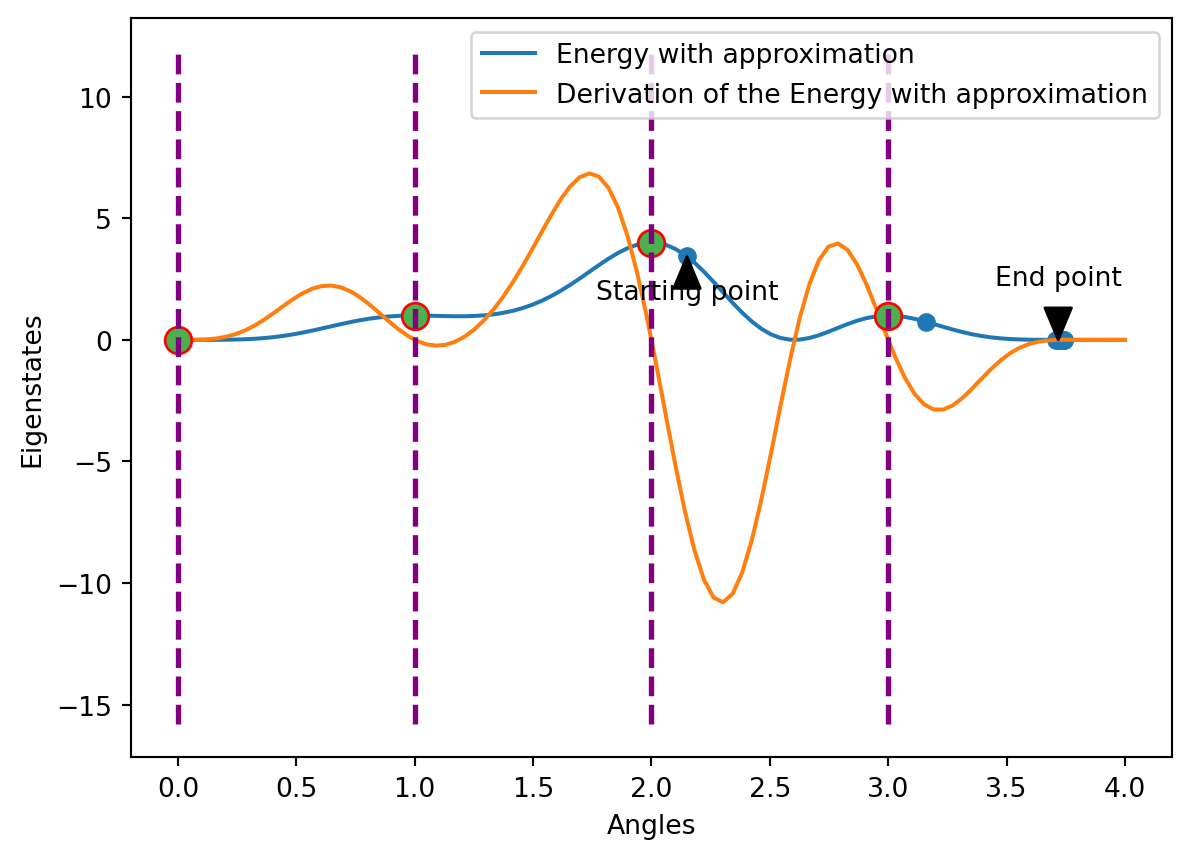
\includegraphics{Optimization_Approximation.png}

}

\caption{\label{fig-surus}Energy graph}

\end{figure}%

\end{minipage}%
%
\begin{minipage}{0.50\linewidth}

\begin{figure}[H]

\centering{

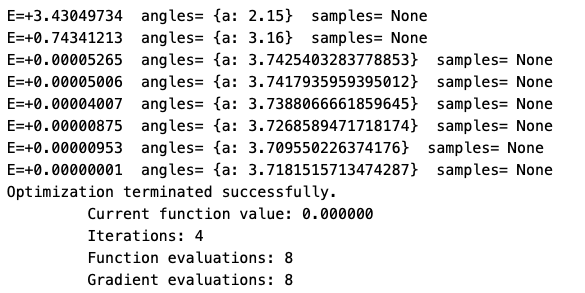
\includegraphics{Optimization_Approximation_process.png}

}

\caption{\label{fig-hanno}Optimization process}

\end{figure}%

\end{minipage}%
\newline
\begin{minipage}{0.50\linewidth}
Optimization with the Approximation method\end{minipage}%

\end{figure}%

First, we start our optimization at Angle 2.15. The blue graph shows us
the energy curve after applying the approximation method, the orange one
the corresponding gradient. Analyzing this, there is a decline in energy
at the starting point, as the orange graph is below the 0 energy level.
According to the optimization procedure, we now the curve until we reach
a local minimum (obervable along the blue dots). In our case, we reach
the local minimum after 7 steps at angle 3.7.

\begin{figure}

\begin{minipage}{0.50\linewidth}

\begin{figure}[H]

\centering{

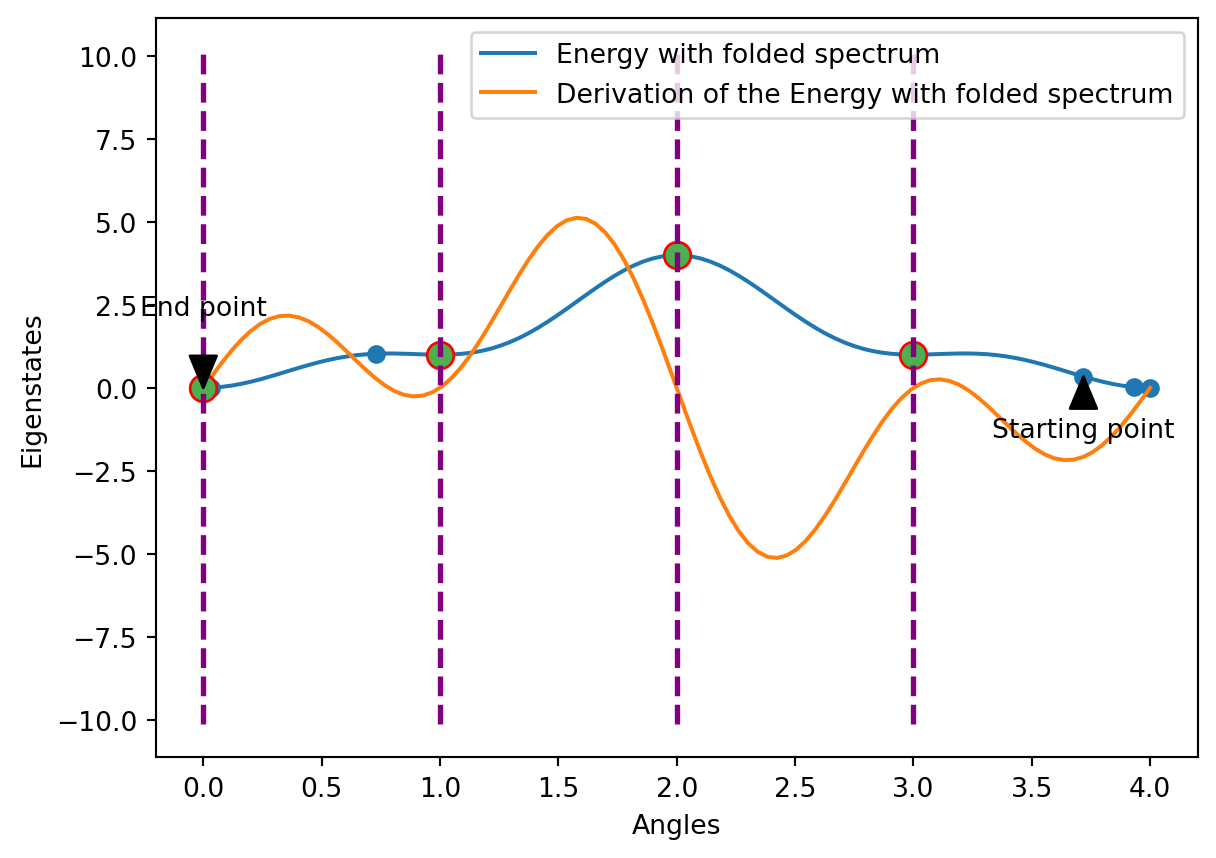
\includegraphics{Optimization_Folded_Spectrum.png}

}

\caption{\label{fig-surus}Energy graph}

\end{figure}%

\end{minipage}%
%
\begin{minipage}{0.50\linewidth}

\begin{figure}[H]

\centering{

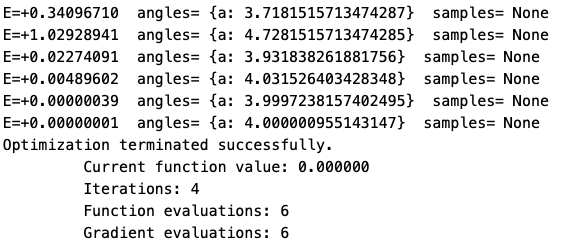
\includegraphics{Optimization_Folded_Spectrum_process.png}

}

\caption{\label{fig-hanno}Optimization process}

\end{figure}%

\end{minipage}%
\newline
\begin{minipage}{0.50\linewidth}
Optimization with the Folded Spectrum method\end{minipage}%

\end{figure}%

This is now the starting point of the Folded Spectrum method. The graph
has changed here: We can see that the gradient at the start is much
lower than the one of the approximation curve at this angle. This means
that there is a point that is even lower than the one previously
assumed. Therefore, we carry out the same procedure as before: we
continue until we arrive at a local minimum again. Since our
optimization steps run in the right direction and in this case we always
consider the angles modulo 4, we end up on the left side again. The
apparent minimum at 0.0 is initially skipped in step 2 and since then we
have been oscillating around the local minimum. In the last step,
however, we return there and remain there. Now we have found an actual
Eigenstate at angle 0.0.

\begin{figure}

\begin{minipage}{0.33\linewidth}

\begin{figure}[H]

\centering{

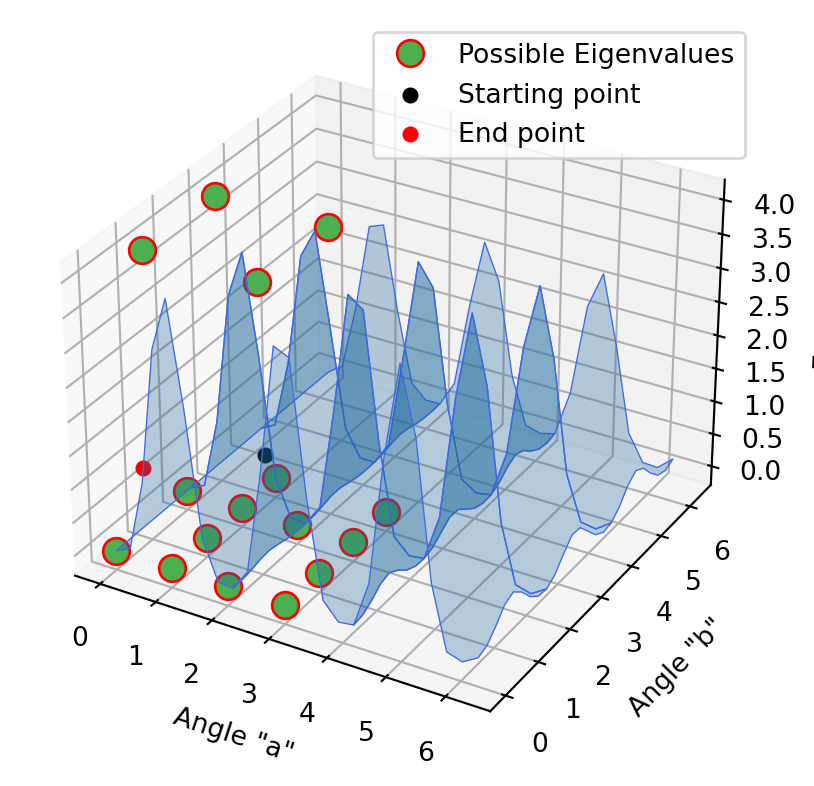
\includegraphics{Approximation_2D.png}

}

\caption{\label{fig-surus}Approximation}

\end{figure}%

\end{minipage}%
%
\begin{minipage}{0.33\linewidth}

\begin{figure}[H]

\centering{

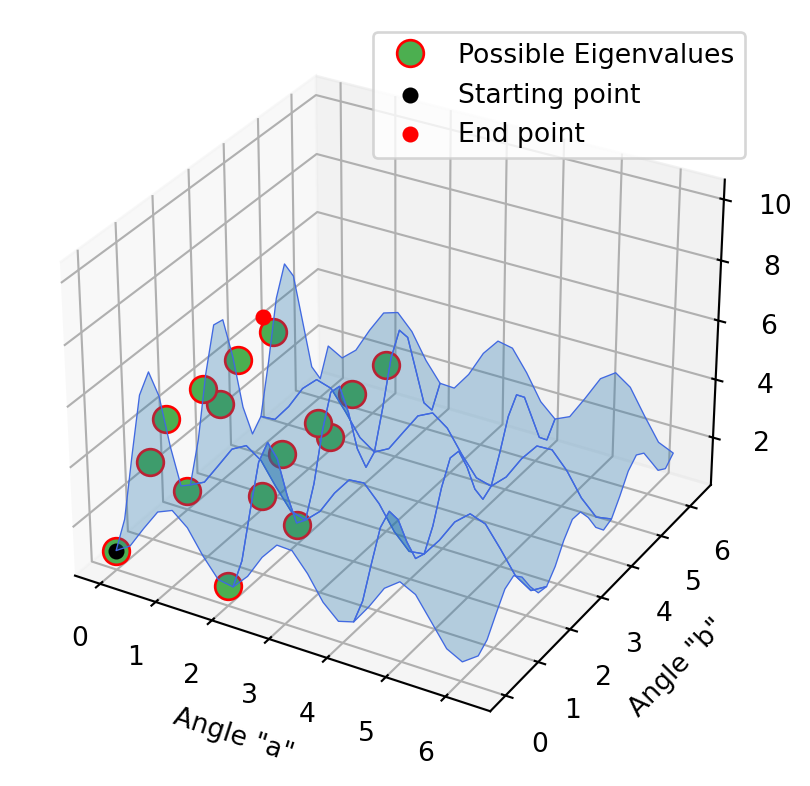
\includegraphics{Projection_2D.png}

}

\caption{\label{fig-hanno}Projection}

\end{figure}%

\end{minipage}%
%
\begin{minipage}{0.33\linewidth}

\begin{figure}[H]

\centering{

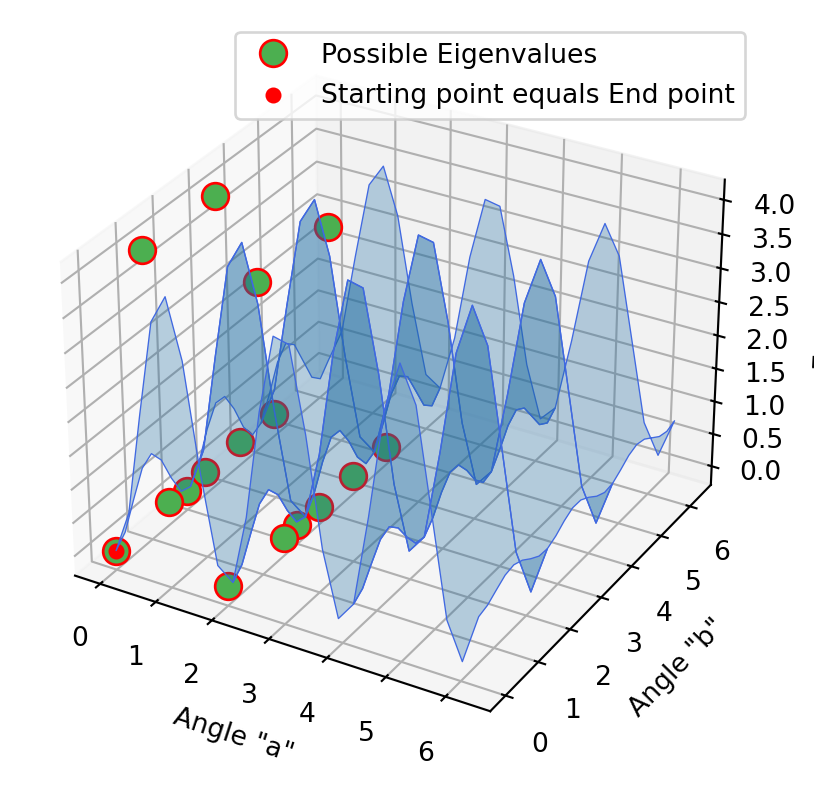
\includegraphics{Folded_spectrum_2D.png}

}

\caption{\label{fig-hanno}Folded Spectrum}

\end{figure}%

\end{minipage}%
\newline
\begin{minipage}{0.33\linewidth}
Optimization with 2D models\end{minipage}%

\end{figure}%

The same procedure was carried out in these 2D models. First with the
approximation method, then the projection method and at the end the
folded spectrum method. It is not initially clear that the end point of
the first method is the starting point of the second method. In fact,
this is the case, only the curves have changed accordingly when the
projection method has been applied. In the second diagram it is already
clear that we have reached a possible Eigenvalue. This is evident in the
last excited state method, since the optimization point does not move,
but stagnates at the minimum.

\section{Conclusion}\label{conclusion}

In summary, this tutorial has provided an overview of quantum
Eigensolvers, a powerful tool for finding the Eigenvalues of quantum
systems. We have discussed the key concepts, such as Hamiltonians,
expectation values, and excited state methods. The Tequila library was
used to implement these concepts and demonstrate their application.
Building on this, we have gained some direct optimization protocols by
testing different concatenations of our excited state methods, including
the optimization after each of them.

Despite this, we need to take some potential errors, such as hardware
errors, which can cause noise, computational errors or Ansatz errors
into consideration. Moreover the accuracy and efficiency of our
Eigensolver depends highly on the choice of our given excited state
methods. Of course, there are also other possibilities of
concatenations, since we have a lot of freedom in selecting the suitable
parameters and order of our introduced techniques.

Overall, by addressing these challenges and leveraging future
advancements, quantum Eigensolvers have the potential to become a
valuable tool for solving complex problems in quantum computing and
beyond.

\subsubsection{Further Reading}\label{further-reading}

\begin{itemize}
\tightlist
\item
  \url{https://pubs.acs.org/doi/epdf/10.1021/acs.jctc.3c01378?ref=article_openPDF}
\item
  \url{https://www.sciencedirect.com/science/article/pii/S0370157322003118?ref=pdf_download&fr=RR-2&rr=8d2f7feaefd39247}
\item
  \url{https://arxiv.org/pdf/1805.08138}
\end{itemize}


\printbibliography


\end{document}
